\section{Kinematics of slow dark matter}\label{sec:1.3}

A dark-matter particle that crosses a detector carries at most \SI{3.5}{eV} of kinetic energy at \SI{1}{MeV} and \SI{3.5}{meV} at \SI{1}{keV}, and about a seventh of that at a typical speed (\cref{sec:1.1}). Whether it can excite a target, and which excitation it can excite, is decided by energy and momentum conservation before any matrix element is computed. Sign conventions follow \cref{app:A.4}.

\subsection{Energy transfer and minimum velocity}

We start from the elastic collision with a free particle at rest. A dark-matter particle of mass $\mchi$ and laboratory velocity $\vect{v}$ has momentum $\mchi\vect{v}$ and kinetic energy $\tfrac12\mchi v^2$; at speeds $v \lesssim 3\times10^{-3}$ the nonrelativistic forms are exact to a part in $10^5$. It scatters on a nucleus of mass $M$ at rest. We write $\vect{q}$ for the momentum transferred \emph{from} the dark matter \emph{to} the target; the dark matter leaves with $\mchi\vect{v} - \vect{q}$ and the nucleus with $\vect{q}$. In a crystal, $\vect{q}$ brings some lattice vocabulary with it; \cref{sec:3.1} develops it properly, and for now four working definitions are enough. A \emph{reciprocal-lattice vector} $\vect{G}$ is a wavevector whose plane wave $\ee^{\ii\vect{G}\cdot\vect{x}}$ takes the same value at every lattice site, and a crystal conserves momentum only up to such a vector. As a result, a state of an electron or phonon in a crystal is labeled by a \emph{crystal momentum}, defined only up to a reciprocal-lattice vector. The \emph{first Brillouin zone} is the set of wavevectors closer to the origin than to any nonzero $\vect{G}$, and \emph{folding} a momentum means subtracting the $\vect{G}$ that brings it into that zone. We never fold $\vect{q}$: it is the physical momentum lost by the dark matter (the reason is given below \cref{eq:1.3-q0}). Energy conservation reads
\begin{equation}
  \tfrac12\mchi v^2 = \frac{(\mchi\vect{v} - \vect{q})^2}{2\mchi} + \frac{q^2}{2M}
  \quad\Longrightarrow\quad
  \vect{q}\cdot\vect{v} = \frac{q^2}{2\mu_{\chi N}},
  \label{eq:1.3-elastic}
\end{equation}
with $q = |\vect{q}|$ and $\mu_{\chi N} = \mchi M/(\mchi + M)$ the dark-matter--nucleus reduced mass~\cite[Eqs.~(75)--(77)]{lin2019tasi}. We write $\mu_{\chi e}$ and $\mu_{\chi p}$ for the reduced masses with an electron and a proton, defined in the same way. Since $\vect{q}\cdot\vect{v} \le qv$, there is a maximum momentum transfer, $q \le 2\mu_{\chi N}v$, and the energy deposited in the nucleus, the \emph{nuclear recoil energy} $E_R = q^2/2M$, obeys~\cite[Eq.~(78)]{lin2019tasi}
\begin{equation}
  E_R \le \frac{2\mu_{\chi N}^2 v^2}{M}.
  \label{eq:1.3-ERmax}
\end{equation}
For $\mchi \ll M$ it is $(4\mchi/M)\times\tfrac12\mchi v^2$: a light particle bounces off a heavy nucleus like a ball off a wall and keeps almost all of its energy.

The free particle at rest is an idealization, and in a solid a poor one: electrons are bound, with typical momenta $\sim \alpha m_e$, and nuclei are tied to a lattice. The target can absorb a momentum $\vect{q}$ and an energy $\omega$ that are not related by a free dispersion $q^2/2M$, and it pays to separate the two parties. We write $\omega$ for the \emph{energy deposited} in the target. In this book it is defined as the energy given to the target, so it can be negative at $T > 0$. All of the target's physics then sits in which pairs $(\vect{q}, \omega)$ it can absorb, and how often. The dark-matter side alone fixes $\omega$ once $\vect{q}$ and $\vect{v}$ are given.

To keep the models of \cref{sec:1.4} in view we allow the scattering to change the dark-matter state, $\chi_1 \to \chi_2$, with a mass splitting $\Delta_\chi = m_{\chi_2} - m_{\chi_1}$. The energy the dark matter loses is its initial kinetic energy minus its final kinetic and extra rest energy:
\begin{equation*}
  \omega = \tfrac12\mchi v^2 - \frac{(\mchi\vect{v} - \vect{q})^2}{2\mchi} - \Delta_\chi .
\end{equation*}
We have neglected $\Delta_\chi$ against $\mchi$ in the final kinetic energy, a relative error $|\Delta_\chi|/\mchi$, negligible for splittings small compared with the mass. Expanding the square, the terms $\tfrac12\mchi v^2$ cancel, and energy conservation becomes $\omega = \omega_{\vect{q}}$, with
\begin{keyresult}[Energy transfer and minimum velocity]
\begin{equation}
  \omega_{\vect{q}} = \vect{q}\cdot\vect{v} - \frac{q^2}{2\mchi} - \Delta_\chi ,
  \label{eq:1.3-omegaq}
\end{equation}
\begin{equation}
  \vmin(q, \omega) = \left|\frac{\omega + \Delta_\chi}{q} + \frac{q}{2\mchi}\right| .
  \label{eq:1.3-vmin}
\end{equation}
A pair $(\vect{q}, \omega)$ is open to a particle of speed $v$ if and only if $v \ge \vmin(q, \omega)$.
\end{keyresult}
\noindent \Cref{eq:1.3-omegaq} is the form used for electron and phonon targets~\cites[Eq.~(9)]{kahn2022searches}[Eq.~(116)]{lin2019tasi}[Eq.~(3.2)]{essig2016direct}. The splitting is endothermic for $\Delta_\chi > 0$, when part of the kinetic energy is spent on the heavier final state, and exothermic for $\Delta_\chi < 0$, when the dark matter releases $|\Delta_\chi|$. For elastic scattering $\Delta_\chi = 0$. A free nucleus at rest absorbs only $\omega = q^2/2M$, and \cref{eq:1.3-omegaq} with $\Delta_\chi = 0$ then returns \cref{eq:1.3-elastic}. Some papers take $\vect{q}$ as the momentum gained by the dark matter instead, a difference that matters for a crystal without inversion symmetry or with magnetic order, where $\vect{q}$ and $-\vect{q}$ are physically different (\cref{app:A.4}).

Bound electrons show why the separation is needed. Treat an outer electron as free but moving with a typical velocity $\sim \alpha$, about ten times faster than the dark matter. Its momentum is then $\sim \alpha m_e$, and a momentum transfer of that size is what changes its state. The typical momentum transfer is set by the electron, not by the dark matter: $q \approx \mu_{\chi e}\alpha$, which is $\alpha m_e$ for $\mchi \gg m_e$~\cite[Eqs.~(117) and (118)]{lin2019tasi}. By \cref{eq:1.3-omegaq} the energy deposited is then $\sim qv \approx \alpha m_e v \approx \SI{4}{eV}$ at $v = 10^{-3}$, independent of $\mchi$, and is not tied to $q$ by any dispersion of the dark matter. For $\mchi < m_e$ the estimate $q \approx \mchi\alpha$ fails: with $\Delta_\chi = 0$, \cref{eq:1.3-omegaq} would allow at most $qv - q^2/2\mchi = \mchi\alpha(v - \alpha/2)$, which is negative because $\alpha/2 = \num{3.6e-3}$ exceeds every halo speed. The momentum transfer is then bounded by roughly $\mchi v$, and the dark matter can give up at most its kinetic energy~\cite[Eq.~(119)]{lin2019tasi}. A real target has a spectrum of states rather than a single electron velocity, and \cref{eq:1.3-omegaq} holds for all of them: it constrains only the dark-matter side.

The minimum velocity follows from the angle. Let $\theta$ be the angle between $\vect{q}$ and $\vect{v}$. \Cref{eq:1.3-omegaq} with $\omega = \omega_{\vect{q}}$ fixes
\begin{equation*}
  \cos\theta = \frac{1}{v}\left(\frac{\omega + \Delta_\chi}{q} + \frac{q}{2\mchi}\right),
\end{equation*}
and a direction with this cosine exists only if the right side lies between $-1$ and $1$. That is the condition $v \ge \vmin$ of \cref{eq:1.3-vmin}. The absolute value matters only when $\omega + \Delta_\chi < 0$, which happens in two cases: for exothermic dark matter, and for a target at temperature $T > 0$ that gives energy to the dark matter, $\omega < 0$ (the thermal weights of such transitions are set in \cref{sec:2.5}). For $\omega + \Delta_\chi < 0$ the signed expression can be negative, and reading a negative value as ``every particle qualifies'' would be wrong: at $\omega = 0$ and small $q$, \cref{eq:1.3-vmin} demands $v \ge |\Delta_\chi|/q$, which no halo particle meets once $q < |\Delta_\chi|/v_{\mathrm{max}}$. With the absolute value, $\vmin \ge 0$ always. At $\omega = -\Delta_\chi = |\Delta_\chi|$ it reduces to $q/2\mchi$, which vanishes as $q \to 0$: an exothermic particle deposits its splitting at any speed, the case of the exothermic models of \cref{sec:1.4}.

Without any knowledge of the target, \cref{eq:1.3-omegaq} fixes the largest energy a particle can deposit and the minimum velocity needed to deposit a given energy. First, at fixed $v$, \cref{eq:1.3-omegaq} is largest for $\vect{q}$ parallel to $\vect{v}$ and $q = \mchi v$, where
\begin{equation}
  \omega \le \tfrac12\mchi v^2 - \Delta_\chi .
  \label{eq:1.3-omegamax}
\end{equation}
For elastic scattering the dark matter can give up its entire kinetic energy, provided the target absorbs the momentum $\mchi v$ at that energy~\cite[Eq.~(119)]{lin2019tasi}. A free target of mass $M$ cannot, because part of the energy goes into its recoil: the most energy that can go into an internal excitation of a free target is $\tfrac12\mu_{\chi T}v^2$, with $\mu_{\chi T}$ the reduced mass of the pair~\cite[Eq.~(3.4)]{essig2016direct}. A crystal absorbs momentum as a whole, its mass is macroscopic, and the full kinetic energy is available. Second, for elastic scattering at fixed $\omega > 0$, \cref{eq:1.3-vmin} as a function of $q$ is smallest where its derivative $-\omega/q^2 + 1/2\mchi$ vanishes, at $q = (2\mchi\omega)^{1/2}$, with the value $\vmin = (2\omega/\mchi)^{1/2}$. A particle of speed $v$ can deposit $\omega$ at some $q$ only if $\tfrac12\mchi v^2 \ge \omega$.

\subsection{Threshold mass}

A detector registers an event only if the deposited energy exceeds a \emph{threshold energy} $E_{\mathrm{th}}$, set by the target (the lowest excitation energy) or by the readout. No particle in the laboratory is faster than $v_{\mathrm{max}} = \SI{794.5}{km.s^{-1}} = 2.650\times10^{-3}$ (\cref{eq:1.2-vmax}). Combining with \cref{eq:1.3-omegamax}, an elastic scatter above threshold requires $\tfrac12\mchi v_{\mathrm{max}}^2 \ge E_{\mathrm{th}}$, that is $\mchi \ge m_{\mathrm{min}}$ with the \emph{threshold mass}
\begin{equation}
  m_{\mathrm{min}} = \frac{2E_{\mathrm{th}}}{v_{\mathrm{max}}^2} .
  \label{eq:1.3-mmin}
\end{equation}
The bound is attained only if the target has an excitation of energy $E_{\mathrm{th}}$ at the momentum $q = m_{\mathrm{min}}v_{\mathrm{max}}$. If the lowest excitation energy of the target depends on $q$, the condition becomes the requirement that $\vmin(q, \omega) \le v_{\mathrm{max}}$ for some $q$ at which the target can absorb $\omega \ge E_{\mathrm{th}}$; \cref{eq:1.3-mmin} with the global minimum of the excitation energy is then a strict lower bound. \Cref{sec:3.3} applies this to silicon, whose lowest electronic excitations sit at a nonzero crystal momentum. For inelastic dark matter $E_{\mathrm{th}}$ is replaced by $E_{\mathrm{th}} + \Delta_\chi$ when this is positive; if $E_{\mathrm{th}} + \Delta_\chi \le 0$, kinematics alone sets no lower mass. The two signs change the spectrum in opposite ways. An endothermic splitting removes $\Delta_\chi$ from every deposit and raises $m_{\mathrm{min}}$. An exothermic splitting adds $|\Delta_\chi|$: by \cref{eq:1.3-omegaq} the deposits then lie between $|\Delta_\chi| - qv - q^2/2\mchi$ and $|\Delta_\chi| + qv - q^2/2\mchi$, a band of width $2qv$ about $|\Delta_\chi|$, and for small $q$ the spectrum approaches a line at the splitting.

The scale of $m_{\mathrm{min}}$ follows from $v_{\mathrm{max}}^2 = 7.02\times10^{-6}$. A threshold of \SI{1}{eV} needs $\mchi \ge \SI{0.28}{MeV}$, and a threshold of \SI{1}{meV} needs $\mchi \ge \SI{0.28}{keV}$. Every factor of ten in threshold is a factor of ten in reach. The threshold mass depends on the halo through $v_{\mathrm{max}}^2$ alone. A shift of the escape speed by \SI{25}{km.s^{-1}}, the size of its uncertainty (\cref{sec:1.2}), changes $v_{\mathrm{max}}$ by \SI{3.1}{\percent} and $m_{\mathrm{min}}$ by \SI{6.3}{\percent}. Over the year the largest speed moves between 781 and \SI{810}{km.s^{-1}} (\cref{eq:1.2-vmax}), and the threshold mass computed with it moves by \SI{-3.9}{\percent} in June and \SI{+3.4}{\percent} in December about its reference value.

\begin{workedexample}{Threshold masses for an electronic and a phonon threshold}\label{we:1-mmin}
The band gap of silicon, the lowest energy that frees an electron from the occupied states, depends on temperature: it is \SI{1.12}{eV} at \SI{300}{K}~\cite[Table~I]{ramanathan2020ionization} and $\SI{1.1692}{eV}$ near zero temperature~\cite[Eq.~(11)]{ramanathan2020ionization}, where detectors run. With the low-temperature gap, $\Eg = \SI{1.17}{eV}$, as the threshold, \cref{eq:1.3-mmin} gives
\begin{equation*}
  m_{\mathrm{min}} = \frac{2 \times \SI{1.17}{eV}}{(2.650\times10^{-3})^2} = \frac{\SI{2.34}{eV}}{\num{7.023e-6}} = \SI{3.33e5}{eV} = \SI{0.333}{MeV}.
\end{equation*}
The optimal momentum transfer is $q = m_{\mathrm{min}}v_{\mathrm{max}} = \SI{3.33e5}{eV}\times 2.650\times10^{-3} = \SI{0.88}{keV}$. \Cref{sec:3.3} computes the gap. For a phonon threshold of \SI{30}{meV},
\begin{equation*}
  m_{\mathrm{min}} = \frac{2 \times \SI{0.030}{eV}}{\num{7.023e-6}} = \SI{8.5e3}{eV} = \SI{8.5}{keV},
\end{equation*}
at $q = \SI{8.5e3}{eV}\times 2.650\times10^{-3} = \SI{23}{eV}$. Lowering the threshold from the electronic to the phonon scale lowers the reach by a factor of $1.17/0.030 = 39$. Both values are limits set by kinematics alone: at $\mchi = m_{\mathrm{min}}$ only particles moving at exactly $v_{\mathrm{max}}$ in exactly the right direction contribute, and the rate vanishes (\cref{sec:1.3-edge}).
\end{workedexample}

\subsection{Momentum and energy scales}

\Cref{eq:1.3-omegaq} defines, for each mass, the region of the $(q, \omega)$ plane that the halo can reach. With $\Delta_\chi = 0$ and the fastest particles moving along $\vect{q}$,
\begin{equation}
  \omega \le q v_{\mathrm{max}} - \frac{q^2}{2\mchi} .
  \label{eq:1.3-region}
\end{equation}
The boundary is a parabola that leaves the origin with slope $v_{\mathrm{max}}$, peaks at $\omega = \tfrac12\mchi v_{\mathrm{max}}^2$ at $q = \mchi v_{\mathrm{max}}$, and returns to zero at $q = 2\mchi v_{\mathrm{max}}$, the maximum momentum transfer. Whatever the mass, every allowed point lies below the line $\omega = qv_{\mathrm{max}}$, and depositing $\omega$ needs $q \ge \omega/v_{\mathrm{max}}$~\cite[Eq.~(122)]{kahn2022searches}; no point lies beyond $q = 2\mchi v_{\mathrm{max}}$. \Cref{fig:1-kinematics} draws the region for four masses, after Ref.~\cite[Fig.~1]{kahn2022searches}, and \cref{tab:1-kinematics} lists the corresponding extremes. The energy deposited is small compared with the momentum transfer, $\omega \le qv_{\mathrm{max}} < 3\times10^{-3}q$. As a result, scattering of halo dark matter is always far from the light cone $\omega = q$, which is why the static potential of \cref{sec:1.4} suffices.

\begin{figure}[tbp]
  \centering
  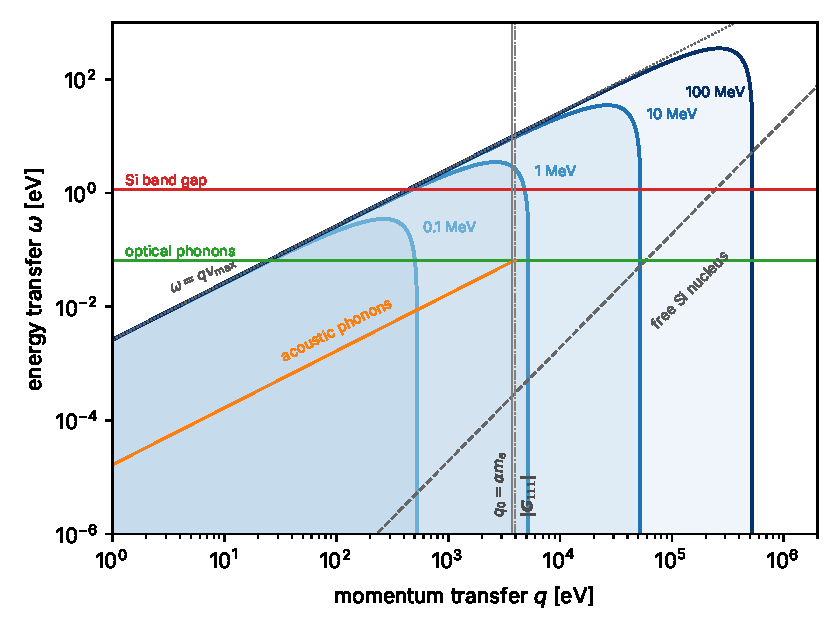
\includegraphics[width=0.9\linewidth]{figures/ch01/fig1_5.pdf}
  \caption{Momentum transfer $q$ and energy transfer $\omega$ accessible to elastic dark matter of mass 0.1, 1, 10 and \SI{100}{MeV} (blue curves, light to dark; shaded below), from $\omega \le qv_{\mathrm{max}} - q^2/2\mchi$ with $v_{\mathrm{max}} = \SI{794.5}{km.s^{-1}}$. The dotted line $\omega = qv_{\mathrm{max}}$ bounds all masses. Overlaid for silicon are the low-temperature band gap, \SI{1.17}{eV} (red), and the optical-phonon energy at the zone center, \SI{64}{meV} (green). The orange line is an acoustic branch $\omega$ = sound speed $\times\,q$ for a sound speed of \SI{5}{km.s^{-1}}, drawn up to $q = |\vect{G}_{111}|$, and the dashed curve is the recoil $q^2/2M$ of a free silicon nucleus, with $M = \SI{26.16}{GeV}$ the mean atomic mass of natural silicon. Vertical lines: the electron momentum scale $q_0 = \alpha m_e = \SI{3.73}{keV}$ and the length $|\vect{G}_{111}| = \sqrt{3}\,2\pi/a \approx \SI{4.0}{keV}$ of the shortest reciprocal-lattice vector of silicon, whose lattice constant is $a = 5.431$\,\AA. Scales from Refs.~\cites[Eqs.~(50) and (121), Sect.~IV\,A]{kahn2022searches}[Eq.~(11)]{ramanathan2020ionization}[lattice parameter of silicon]{mohr2025codata}.}
  \label{fig:1-kinematics}
\end{figure}

\begin{table}[tbp]
  \centering
  \caption{Kinematic extremes for elastic dark matter at $v_{\mathrm{max}} = \SI{794.5}{km.s^{-1}}$. Columns: the dark-matter mass; the largest momentum transfer to a target that absorbs any momentum; the largest energy transfer; the largest recoil energy of a free silicon nucleus ($M = \SI{26.16}{GeV}$, the mean atomic mass of natural silicon). The $\tfrac12\mchi v_{\mathrm{max}}^2$ column is also the threshold energy for which $m_{\mathrm{min}} = \mchi$.}
  \label{tab:1-kinematics}
  \begin{tabular}{@{}rrrr@{}}
    \toprule
    $\mchi$ & $2\mchi v_{\mathrm{max}}$ & $\tfrac12\mchi v_{\mathrm{max}}^2$ & free Si nucleus \\
    \midrule
    \SI{0.1}{MeV} & \SI{0.53}{keV} & \SI{0.35}{eV} & \SI{5.4}{\micro eV} \\
    \SI{1}{MeV} & \SI{5.3}{keV} & \SI{3.5}{eV} & \SI{0.54}{meV} \\
    \SI{10}{MeV} & \SI{53}{keV} & \SI{35}{eV} & \SI{54}{meV} \\
    \SI{100}{MeV} & \SI{530}{keV} & \SI{351}{eV} & \SI{5.3}{eV} \\
    \SI{1}{GeV} & \SI{5.3}{MeV} & \SI{3.5}{keV} & \SI{0.50}{keV} \\
    \bottomrule
  \end{tabular}
\end{table}

\Cref{fig:1-kinematics} answers at a glance which excitations each mass can reach. At \SI{0.1}{MeV} the largest deposit, \SI{0.35}{eV}, is below the silicon gap: only phonons, and other excitations below an eV, are open. At \SI{1}{MeV} the gap is open in a narrow band of momentum transfers, from $q = \SI{0.49}{keV}$ to \SI{4.8}{keV}, the two roots of \cref{eq:1.3-region} at $\omega = \SI{1.17}{eV}$. At \SI{10}{MeV} the band widens to 0.45--\SI{53}{keV}, and deposits up to \SI{35}{eV} are allowed. A free silicon nucleus, by contrast, receives \SI{1.17}{eV} only for $\mchi \gtrsim \SI{47}{MeV}$, where $2\mu_{\chi N}^2v_{\mathrm{max}}^2/M$ reaches that value.

Two momentum scales of the target, one for bound electrons and one for the lattice, decide what these momentum transfers probe. The first is the \emph{electron momentum scale}
\begin{equation}
  q_0 = \alpha m_e = \SI{3.73}{keV},
  \label{eq:1.3-q0}
\end{equation}
the inverse Bohr radius~\cite[Eq.~(121)]{kahn2022searches}. A bound outer electron has a wavefunction of size $1/(\alpha m_e)$ and typical momenta $\sim q_0$~\cite[Sect.~V\,A]{lin2019tasi}. A momentum transfer much smaller than $q_0$ barely changes the electron's state; a much larger one reaches only the high-momentum tail of its wavefunction. The second is the \emph{interatomic scale}, the length of the shortest reciprocal-lattice vector. For a cubic crystal with lattice constant $a$ the natural unit is $2\pi/a$. Silicon has $a = 5.431$\,\AA~\cite[lattice parameter of silicon]{mohr2025codata}, about ten Bohr radii~\cite[Sect.~V]{kahn2022searches}, which makes $2\pi/a = \SI{2.28}{keV} = 0.61\,q_0$. Its lattice is face-centered cubic, and the shortest reciprocal-lattice vectors, along the cube diagonals, are longer by $\sqrt{3}$: $|\vect{G}_{111}| = \sqrt{3}\,2\pi/a = \SI{3.95}{keV} \approx 1.06\,q_0$. A momentum transfer well below $|\vect{G}_{111}|$ has a wavelength longer than the interatomic spacing and sees the crystal as a whole; a larger one resolves the atoms. \Cref{sec:3.1} makes this precise with the reciprocal lattice.

The two scales are close to each other, and light dark matter straddles both. For an electronic excitation of a few eV, $q \ge \omega/v_{\mathrm{max}}$ requires $q \gtrsim \SI{1}{keV}$, roughly $0.3\,q_0$; the silicon gap alone needs $q \ge \SI{1.17}{eV}/2.650\times10^{-3} = \SI{0.44}{keV} = 0.12\,q_0$~\cite[Eq.~(123)]{kahn2022searches}. At the upper end, interpolating \cref{tab:1-kinematics}, $2\mchi v_{\mathrm{max}} = q_0$ at $\mchi = \SI{0.70}{MeV}$. Between about \SI{1}{MeV} and \SI{1}{GeV}, then, the momentum transfers match the momenta at which electrons in atoms and solids have most of their weight. Lighter dark matter cannot reach $q_0$ and probes the long-wavelength response of the crystal. Heavier dark matter can reach far above $q_0$, but momentum transfers of that size find little electronic weight.

The comparison with $|\vect{G}_{111}|$ explains why we never fold $\vect{q}$. Above about \SI{0.75}{MeV}, $2\mchi v_{\mathrm{max}}$ exceeds $|\vect{G}_{111}|$. Because the crystal conserves momentum only up to a reciprocal-lattice vector, the same excitation can be reached by momentum transfers that differ by such a vector, and these have different magnitudes. The dark-matter side, \cref{eq:1.3-omegaq,eq:1.3-vmin}, depends on the magnitude of the physical momentum transfer $\vect{q}$, not on its image in the first Brillouin zone. Folding $\vect{q}$ would assign the wrong $\vmin$ and the wrong dark-matter form factor $\FDM(q)$ of \cref{sec:1.4}. \Cref{sec:3.1} writes $\vect{q}$ as a first-zone part plus a reciprocal-lattice vector and keeps both.

On the energy side, electronic excitations and phonons set the scales. \emph{Electronic excitations} move an electron from an occupied to an empty state and typically cost an eV or more. In an insulator or semiconductor the lowest such energy is the \emph{band gap} $\Eg$ (\cref{we:1-mmin}; \cref{sec:3.3}). \emph{Phonons} are the quantized vibrations of the lattice, with energies from zero to roughly \SI{100}{meV}~\cite[Sect.~III\,A]{kahn2022searches}; the optical phonon of silicon at the zone center has \SI{64}{meV}, or \SI{15.5}{THz}~\cite{nilsson1972study} (\cref{sec:5.3}). Two kinds, optical and acoustic, matter here. Optical phonons, in which neighboring atoms move against each other, keep a finite energy as their momentum goes to zero. Acoustic phonons, long-wavelength sound waves, have energy equal to the sound speed times the momentum, with sound speeds of 3 to \SI{10}{km.s^{-1}}~\cite[Eq.~(50)]{kahn2022searches}, that is $1$ to $3\times10^{-5}$.

The kinematics treats optical and acoustic phonons differently. An optical phonon branch that is nearly flat, with energy $\omega$, can be excited at any $q$ between $\omega/v_{\mathrm{max}}$ and the upper root of \cref{eq:1.3-region}, close to $2\mchi v_{\mathrm{max}}$. Such a branch can absorb nearly the full kinetic energy, and \cref{eq:1.3-mmin} applies; the \SI{30}{meV} threshold of \cref{we:1-mmin} needs a momentum transfer of just $q \approx \SI{23}{eV}$, below a hundredth of $|\vect{G}_{111}|$. An acoustic phonon of branch $\nu$ has $\omega = c_\nu q$, with $c_\nu$ its sound speed (\cref{sec:5.2}). By \cref{eq:1.3-vmin} it needs $\vmin = c_\nu + q/2\mchi \le v$, which bounds $q \le 2\mchi(v - c_\nu)$ and $\omega \le 2c_\nu\mchi v$ to leading order in $c_\nu/v$~\cite[Eq.~(93)]{kahn2022searches}. The acoustic branch takes at most a fraction $4c_\nu/v$, a few percent, of the kinetic energy. In \cref{fig:1-kinematics} it is the orange line, which for the lightest mass leaves the parabola near its right end.

Both energy scales are material properties, and later chapters use computed values for them. The band gap is computed from first principles with density-functional theory, corrected for the systematic underestimate of gaps that the method makes (\cref{app:E.1,app:E.3}); phonon energies come from density-functional perturbation theory (\cref{app:E.4}). Measured values serve as checks.

\paragraph{Nuclear recoils.} \Cref{eq:1.3-ERmax} shows why scattering on free nuclei loses its reach for light dark matter. The free nucleus is the dashed parabola $\omega = q^2/2M$ of \cref{fig:1-kinematics}. It meets each dark-matter region only where $q^2/2M$ is small, because $M$ is large; for $\mchi \ll M$ the nucleus receives at most the fraction $4\mchi/M$ of the kinetic energy, $\num{1.5e-2}$ at \SI{100}{MeV} on silicon. The same parabola explains when a nucleus in a crystal is not free. A recoil energy comparable to the phonon energies, tens of meV, is reached at $\mchi \approx \SI{10}{MeV}$ (\cref{tab:1-kinematics}). Below that mass the nucleus cannot be treated as free: the dark matter excites one or a few phonons of the crystal instead, with the energies set by the lattice, and \cref{chap:5} develops that description.

For a free nucleus, \cref{eq:1.3-vmin} at $\omega = E_R = q^2/2M$ gives $\vmin = q/2\mu_{\chi N} = (ME_R/2\mu_{\chi N}^2)^{1/2}$. The crossover to phonons is already visible for a single nucleus held in a harmonic well of frequency $\omega_0$. At zero temperature a transfer $q$ excites $n$ quanta with the Poisson probability $P_n = \ee^{-E_R/\omega_0}(E_R/\omega_0)^n/n!$, where $E_R = q^2/2M$ is the free recoil energy~\cite[Eqs.~(90) and (91)]{kahn2022searches}. The energy deposit $n\omega_0$ therefore has mean exactly $E_R$ and rms spread $(E_R\omega_0)^{1/2}$. The free formula is the limit $E_R \gg \omega_0$, in which the spread is small compared with $E_R$.

\begin{limitbox}[Elastic nuclear recoil][lim:1.3a]
A free nucleus of mass $M$ at rest that receives momentum $q$ absorbs the energy $\omega = E_R = q^2/2M$. A dark-matter particle of speed $v$ gives it at most $E_R \le 2\mu_{\chi N}^2v^2/M$, with $\mu_{\chi N}$ the dark-matter--nucleus reduced mass, and a recoil $E_R$ needs the speed $v \ge \vmin = (ME_R/2\mu_{\chi N}^2)^{1/2}$~\cite[Eqs.~(77) and (78)]{lin2019tasi}.
\par\smallskip
{\centering
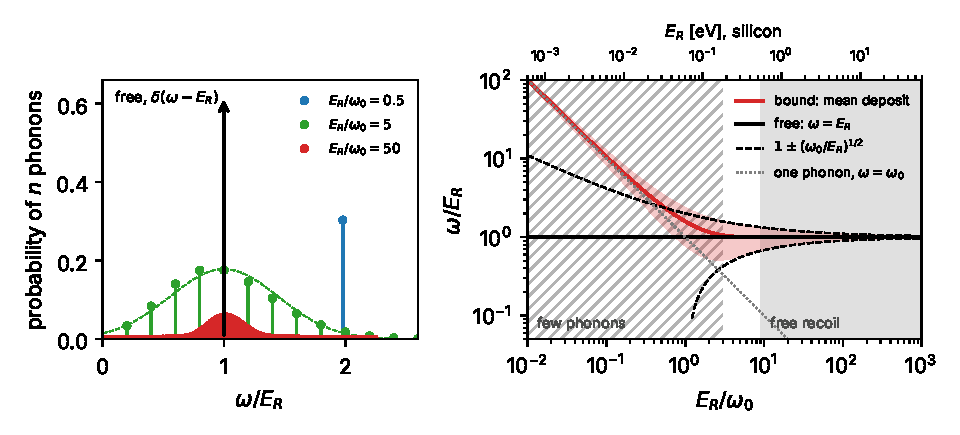
\includegraphics[width=\linewidth]{figures/ch01/limit1_nuclear.pdf}
\captionof{figure}{Free nuclear recoil against a nucleus bound in a harmonic (Einstein) potential of frequency $\omega_0 = \SI{60}{meV}$, a typical silicon phonon energy, at zero temperature~\cite[Sect.~IV\,A, Eqs.~(80), (90) and (91)]{kahn2022searches}. Left: probability of exciting $n$ phonons, a deposit $\omega = n\omega_0$, for $E_R/\omega_0 = 0.5$, 5 and 50 (dots; the term $n = 0$, which deposits nothing, is omitted), with Gaussians of rms width $(E_R\omega_0)^{1/2}$ (dashed) and the free response $\delta(\omega - E_R)$ (arrow). Right: mean deposit of the scatterings that excite the lattice (red line) and its rms spread (red band), against $E_R/\omega_0$, with the free value $\omega = E_R$ (black), the estimate $1 \pm (\omega_0/E_R)^{1/2}$ (dashed) and one phonon, $\omega = \omega_0$ (dotted); the top axis gives $E_R$ for silicon. Gray: $E_R \ge 9\omega_0 = \SI{0.54}{eV}$, where the rms width is below a third of $E_R$ and the free formula holds. Hatched: $E_R \le 3\omega_0$, the single- and few-phonon regime.}\label{fig:1-recoil-limit}
\par}
\smallskip
Below a few $\omega_0$ the deposit comes in whole phonons and spreads as widely as $E_R$ itself; below $\omega_0$ most scatterings leave the lattice unexcited, and the rest deposit at least one phonon, $\omega_0$, well above $E_R$.
\end{limitbox}

\begin{workedexample}{Largest recoil energy of a silicon nucleus}\label{we:1-nuclear}
For $\mchi = \SI{1}{GeV}$ on silicon, $M = \SI{26.16}{GeV}$ (the mean atomic mass of natural silicon) and $\mu_{\chi N} = (1 \times 26.16/27.16)\,\si{GeV} = \SI{0.963}{GeV}$. The maximum momentum transfer at $v_{\mathrm{max}}$ is $q = 2\mu_{\chi N}v_{\mathrm{max}} = 2 \times \SI{0.963}{GeV} \times 2.650\times10^{-3} = \SI{5.10}{MeV}$, and \cref{eq:1.3-ERmax} gives
\begin{equation*}
  E_R = \frac{q^2}{2M} = \frac{(\SI{5.10}{MeV})^2}{2 \times \SI{26160}{MeV}} = \SI{5.0e-4}{MeV} = \SI{0.50}{keV}.
\end{equation*}
The kinetic energy at $v_{\mathrm{max}}$ is $\tfrac12\mchi v_{\mathrm{max}}^2 = \SI{3.5}{keV}$, so the nucleus receives at most \SI{14}{\percent} of it; the exact fraction is $4\mu_{\chi N}^2/(\mchi M) = 0.142$. A typical particle, at $v \approx \SI{300}{km.s^{-1}}$ and with an average over angles, deposits far less. This momentum transfer, \SI{5.1}{MeV}, is below the inverse nuclear radius, tens of MeV, so the nucleus recoils coherently (\cref{sec:1.4}). On xenon, $M = \SI{122.3}{GeV}$, the same formula gives \SI{0.11}{keV}, the value quoted in \cref{sec:1.1}.
\end{workedexample}

\subsection{The speed integral}\label{sec:1.3-eta}

A rate sums the probability of each momentum transfer over the dark-matter velocities. Energy conservation enters it as a delta function $\delta(\omega - \omega_{\vect{q}})$, integrated against $f_\chi(\vect{v})$ (\cref{sec:2.2} derives the rate). The integral over $\vect{v}$ can be done once for all targets whose response depends on the magnitude $q$ but not on the direction of $\vect{q}$, as for a liquid, an atom, or a crystal averaged over orientations. For such a target only the angle $\theta$ between $\vect{q}$ and $\vect{v}$ matters. Its average is
\begin{equation*}
  \frac12\int_{-1}^{1} \dd(\cos\theta)\, \delta\!\left(\omega + \Delta_\chi + \frac{q^2}{2\mchi} - qv\cos\theta\right)
  = \frac{1}{2qv}\,\Theta\!\left(v - \vmin(q, \omega)\right).
\end{equation*}
The delta function fires once if its root $\cos\theta = (\omega + \Delta_\chi + q^2/2\mchi)/qv$ lies in $[-1, 1]$, which is the condition $v \ge \vmin$. The factor $1/qv$ is the derivative of its argument with respect to $\cos\theta$. This is the origin of the factor $1/v$ promised in \cref{sec:1.2}. Averaging over the halo, we find $\int \dd^3 v\, f_\chi(\vect{v})\,\Theta(v - \vmin)/(2qv) = \eta(\vmin)/(2q)$, with
\begin{equation}
  \eta(\vmin) \equiv \int \dd^3 v\, \frac{f_\chi(\vect{v})}{v}\,\Theta(v - \vmin) = \left\langle \frac{\Theta(v - \vmin)}{v}\right\rangle.
  \label{eq:1.3-eta}
\end{equation}
The function $\eta(\vmin)$ is the \emph{mean inverse speed above} $\vmin$. It carries all of the halo dependence of a rate for such a target~\cites[below Eq.~(5)]{essig2012direct}[Eqs.~(11) and (12)]{kahn2022searches}[Eqs.~(A.12)--(A.15)]{essig2016direct}. Its value at zero is the mean inverse speed $\langle 1/v\rangle$ of \cref{eq:1.2-inv}, and it decreases monotonically to zero at the largest speed in the halo. Because $\vmin \ge 0$ by \cref{eq:1.3-vmin}, $\eta$ is never needed at negative arguments.

\Cref{eq:1.3-eta} fixes how the halo enters the integral over momentum transfers. For an integrand that depends only on $q$, $\dd^3q/(2\pi)^3 = 4\pi q^2\dd q/(2\pi)^3$, and with the factor $\eta/2q$ the measure becomes~\cites[Eq.~(11)]{kahn2022searches}[Eq.~(A.14)]{essig2016direct}
\begin{equation*}
  \int\frac{\dd^3 q}{(2\pi)^3}\,\frac{\eta(\vmin)}{2q}\,(\cdots) = \int\frac{q\,\dd q}{4\pi^2}\,\eta\bigl(\vmin(q, \omega)\bigr)\,(\cdots).
\end{equation*}
Small momentum transfers carry the weight $q\,\dd q$, and $\eta$ cuts the integral off wherever $\vmin(q, \omega) > v_{\mathrm{max}}$, at both small and large $q$. \Cref{sec:1.5} assembles the full rate from this measure, the cross-section of \cref{sec:1.4} and the response of the target. For an anisotropic crystal at a fixed orientation the angular average does not factor out; the rate then depends on the direction of $\vect{v}_{\mathrm{E}}$ relative to the crystal axes, which is the daily modulation of \cref{sec:1.2}.

In the standard halo model the integral is elementary. With $F_\chi(v)$ the speed distribution of \cref{eq:1.2-Fspeed}, $\eta(\vmin) = \int_{\vmin}^\infty \dd v\, F_\chi(v)/v$, and the factor $v$ in $F_\chi$ cancels the $1/v$. \Cref{app:D.1} integrates the Gaussians and finds three branches in closed form: \cref{eq:D.1-eta1} for $0 \le \vmin < v_{\mathrm{esc}} - v_{\mathrm{E}}$, \cref{eq:D.1-eta2} for $v_{\mathrm{esc}} - v_{\mathrm{E}} \le \vmin < v_{\mathrm{esc}} + v_{\mathrm{E}}$, and $\eta = 0$ above. Both are differences of error functions (\cref{app:C.8}) minus a constant from the cut, with $v_{\mathrm{E}} = |\vect{v}_{\mathrm{E}}(t)|$.

\Cref{fig:1-eta} shows $\eta$ at the reference Earth speed and on the days of largest and smallest Earth speed. Three features matter for light dark matter: a plateau, a Gaussian fall and a second branch. Up to $\vmin \approx \SI{200}{km.s^{-1}}$, $\eta$ stays within a factor of 1.41 of $\langle 1/v\rangle = 1/(\SI{287.9}{km.s^{-1}})$: almost every particle qualifies. Between 300 and \SI{700}{km.s^{-1}} it falls roughly as a Gaussian, $\ee^{-(\vmin - v_{\mathrm{E}})^2/v_0^2}$, by a factor of 190, from \SI{1.53e-3}{(km/s)^{-1}} to \SI{7.95e-6}{(km/s)^{-1}}. Above $v_{\mathrm{esc}} - v_{\mathrm{E}}^{\mathrm{ref}} = \SI{293.5}{km.s^{-1}}$ the second branch applies; every $\vmin$ near a kinematic threshold lies on it. In natural units, $\eta(0) = 1041$, $\eta(\SI{600}{km.s^{-1}}) = 19.2$ and $\eta(\SI{700}{km.s^{-1}}) = 2.38$.

\begin{figure}[tbp]
  \centering
  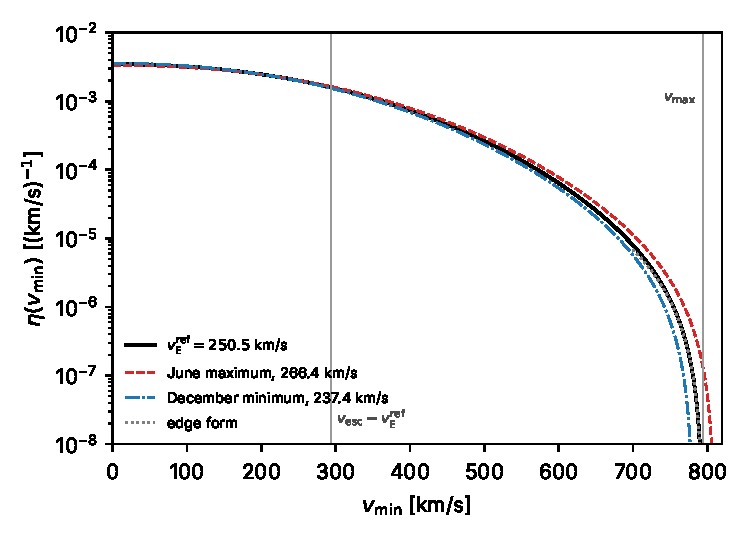
\includegraphics[width=0.8\linewidth]{figures/ch01/fig1_6.pdf}
  \caption{Mean inverse speed above $\vmin$, $\eta(\vmin) = \langle\Theta(v - \vmin)/v\rangle$, in the standard halo model ($v_0 = \SI{238}{km.s^{-1}}$, $v_{\mathrm{esc}} = \SI{544}{km.s^{-1}}$). Solid: Earth speed $v_{\mathrm{E}}^{\mathrm{ref}} = \SI{250.5}{km.s^{-1}}$; dashed: June maximum (\SI{266.4}{km.s^{-1}}); dash-dotted: December minimum (\SI{237.4}{km.s^{-1}}). Vertical lines: $v_{\mathrm{esc}} - v_{\mathrm{E}}^{\mathrm{ref}} = \SI{293.5}{km.s^{-1}}$, where the closed form changes branch, and $v_{\mathrm{max}} = \SI{794.5}{km.s^{-1}}$, where $\eta$ vanishes. The dotted curve above \SI{700}{km.s^{-1}} is the edge form of \cref{eq:1.3-edge} with its first correction; it lies within \SI{10}{\percent} of the exact curve above \SI{720}{km.s^{-1}}, within \SI{5}{\percent} above \SI{745}{km.s^{-1}}, and merges with it toward $v_{\mathrm{max}}$. At $\vmin = 0$, $\eta = 1/(\SI{287.9}{km.s^{-1}})$, or 1041 in natural units. Closed form from \cref{app:D.1}; halo parameters from Ref.~\cite[Table~1]{baxter2021recommended}.}
  \label{fig:1-eta}
\end{figure}

Near the end point the moving cut dominates the seasonal change. Relative to the reference curve, $\eta$ in June and December is 1.42 and 0.72 times as large at $\vmin = \SI{700}{km.s^{-1}}$, 2.2 and 0.37 times at \SI{760}{km.s^{-1}}, and 4.5 and 0.009 times at \SI{780}{km.s^{-1}}, where the December halo has almost no particles left.

\subsection{The kinematic edge}\label{sec:1.3-edge}

The \emph{kinematic edge} of a rate is the boundary beyond which no particle in the halo is fast enough. At fixed $\mchi$ the spectrum ends at $\omega = \tfrac12\mchi v_{\mathrm{max}}^2 - \Delta_\chi$, by \cref{eq:1.3-omegamax}. At a fixed threshold the rate, as a function of mass, ends at $m_{\mathrm{min}}$. Both edges are reached as $\vmin \to v_{\mathrm{max}}$, and the shape of a rate near an edge is controlled by the shape of $\eta$ there.

Close to $v_{\mathrm{max}}$, $\eta$ vanishes as a power. Write $\vmin = v_{\mathrm{esc}} + v_{\mathrm{E}} - \delta$ with small $\delta > 0$. On the second branch, \cref{eq:D.1-eta2}, the difference of error functions is an integral, $(\sqrt{\pi}v_0/2)[\operatorname{erf}(v_{\mathrm{esc}}/v_0) - \operatorname{erf}((v_{\mathrm{esc}} - \delta)/v_0)] = \int_{v_{\mathrm{esc}} - \delta}^{v_{\mathrm{esc}}}\ee^{-y^2/v_0^2}\dd y$, and the constant term is $\delta\,\ee^{-v_{\mathrm{esc}}^2/v_0^2} = \int_{v_{\mathrm{esc}} - \delta}^{v_{\mathrm{esc}}}\ee^{-v_{\mathrm{esc}}^2/v_0^2}\dd y$. With $s = v_{\mathrm{esc}} - y$, the integrand of their difference is
\begin{equation*}
  \ee^{-v_{\mathrm{esc}}^2/v_0^2}\left[\ee^{(2v_{\mathrm{esc}}s - s^2)/v_0^2} - 1\right]
  = \ee^{-v_{\mathrm{esc}}^2/v_0^2}\left[\frac{2v_{\mathrm{esc}}s}{v_0^2} + \left(\frac{2v_{\mathrm{esc}}^2}{v_0^4} - \frac{1}{v_0^2}\right)s^2 + O(s^3)\right].
\end{equation*}
Integrating over $0 < s < \delta$ and multiplying by the prefactor $\pi v_0^2/(v_{\mathrm{E}}N_{\mathrm{esc}})$,
\begin{equation}
  \eta(\vmin) = \frac{\pi v_{\mathrm{esc}}\,\ee^{-v_{\mathrm{esc}}^2/v_0^2}}{v_{\mathrm{E}}N_{\mathrm{esc}}}\,\delta^2\left[1 + \frac{(2v_{\mathrm{esc}}^2 - v_0^2)\,\delta}{3v_{\mathrm{esc}}v_0^2} + O(\delta^2)\right],
  \qquad \delta = v_{\mathrm{esc}} + v_{\mathrm{E}} - \vmin .
  \label{eq:1.3-edge}
\end{equation}
The scale of the correction is $3v_{\mathrm{esc}}v_0^2/(2v_{\mathrm{esc}}^2 - v_0^2) = \SI{173}{km.s^{-1}}$. At the reference Earth speed and $\vmin = 760$ and \SI{780}{km.s^{-1}} ($\delta = 34.5$ and \SI{14.5}{km.s^{-1}}), the quadratic term alone captures 0.81 and 0.92 of the exact value, and with the correction 0.98 and 1.00. The edge is quadratic because two things vanish together: the speed window $v_{\mathrm{max}} - \vmin$, and the density of particles inside it, which drops linearly to zero at the escape speed of the truncated Maxwellian. The prefactor $\ee^{-v_{\mathrm{esc}}^2/v_0^2}/N_{\mathrm{esc}}$ is the height of the distribution at the cut. Both factors are fixed by the most uncertain parts of the halo model (\cref{sec:1.2}); a smoother truncation would raise the power of $\delta$.

The edge in mass follows. For a threshold $E_{\mathrm{th}}$ the smallest $\vmin$ available to a particle of mass $\mchi$ is $(2E_{\mathrm{th}}/\mchi)^{1/2}$ (below \cref{eq:1.3-omegamax}). Its distance from $v_{\mathrm{max}}$ is
\begin{equation*}
  v_{\mathrm{max}} - \left(\frac{2E_{\mathrm{th}}}{\mchi}\right)^{1/2} = v_{\mathrm{max}}\left[1 - \left(\frac{m_{\mathrm{min}}}{\mchi}\right)^{1/2}\right] \simeq \frac{v_{\mathrm{max}}}{2}\,\frac{\mchi - m_{\mathrm{min}}}{m_{\mathrm{min}}},
\end{equation*}
so a mass one percent above $m_{\mathrm{min}}$ uses only particles within \SI{4}{km.s^{-1}} of $v_{\mathrm{max}}$. Just above the edge the rate is the product of $\eta$, quadratic in this window, and of the phase space of pairs $(q, \omega)$ that fit inside it, which shrinks as a further power of the window. How fast that phase space shrinks depends on how the target's response begins at threshold. For silicon the electronic response begins at a crystal momentum away from the zone center, and the question becomes which excitations the dark matter can reach at the edge (\cref{sec:3.3}).

The recovery above the edge is slow. Take the silicon gap of \cref{we:1-mmin} as threshold, $m_{\mathrm{min}} = \SI{0.333}{MeV}$, and evaluate $\eta$ at the most favorable speed $(2\Eg/\mchi)^{1/2}$, an upper bound on what the halo offers at each mass. Relative to $\eta(0)$, it is $\num{6.0e-5}$ at \SI{0.35}{MeV}, $\num{1.1e-3}$ at \SI{0.4}{MeV}, \SI{0.76}{\percent} at \SI{0.5}{MeV}, \SI{12}{\percent} at \SI{1}{MeV} and \SI{84}{\percent} at \SI{10}{MeV}. Between \SI{0.35}{MeV}, \SI{5}{\percent} above $m_{\mathrm{min}}$, and $2m_{\mathrm{min}}$ the halo supply grows by a factor of more than 500. The whole of that range is set by particles faster than about \SI{560}{km.s^{-1}}, the most favorable speed at $2m_{\mathrm{min}}$, which are \SI{7}{\percent} of the halo. A limit in this mass range is a statement about the tail of the velocity distribution as much as about the target.

The position of the edge, by contrast, depends on the target and the halo only through $E_{\mathrm{th}}/v_{\mathrm{max}}^2$. Their uncertainties enter as $\delta\ln m_{\mathrm{min}} = \delta\ln E_{\mathrm{th}} - 2\,\delta\ln v_{\mathrm{max}}$. A \SI{5}{\percent} change in the gap moves $m_{\mathrm{min}}$ by \SI{5}{\percent}.
